\documentclass[12pt, a4paper]{article}

% ==========================================
% 1. KHAI BÁO GÓI THƯ VIỆN (PACKAGES)
% ==========================================
% Bảng mã & Font chữ
\usepackage[utf8]{inputenc}
\usepackage[T5]{fontenc}

% Toán học
\usepackage{amsmath, amssymb}

% Căn lề & Bố cục trang
\usepackage[top=2.2cm, bottom=1.5cm, left=1cm, right=1cm, headheight=15pt]{geometry}
\usepackage{fancyhdr}
\usepackage{needspace}
\usepackage{tkz-tab}

% Đồ họa & Màu sắc
\usepackage{xcolor}
\usepackage{graphicx} 
\usepackage{tikz}
\usetikzlibrary{calc, shapes.geometric, positioning}


% Bảng biểu & Danh sách
\usepackage{colortbl}
\usepackage{array}
\usepackage{makecell}
\usepackage{multirow}
\usepackage{tasks}

% Biểu tượng
\usepackage{fontawesome5}

% ==========================================
% 2. THIẾT LẬP MÀU SẮC CHỦ ĐẠO
% ==========================================
\definecolor{goldyellow}{RGB}{255, 179, 0}
\definecolor{amberorange}{RGB}{230, 115, 0}
\definecolor{lightamber}{RGB}{255, 248, 225}
\definecolor{deepblue}{RGB}{25, 42, 86}
\definecolor{accentred}{RGB}{232, 65, 24}
\definecolor{softgray}{RGB}{220, 220, 222} 
\definecolor{fbblue}{RGB}{15, 80, 200}


% ==========================================
% 3. CẤU HÌNH HEADER & FOOTER
% ==========================================
\pagestyle{fancy}
\fancyhf{}
\renewcommand{\headrulewidth}{0pt}

% Khai báo biến lưu trữ nội dung góc phải của Header
\newcommand{\HeaderRightText}{}

% --- Header ---
\fancyhead[C]{
    \begin{tikzpicture}[remember picture, overlay]
        
        % Dải màu trang trí góc trên
        \path[fill=deepblue] (current page.north west) -- (current page.north east) 
            -- ($(current page.north east) + (0, -1.6cm)$) 
            .. controls ($(current page.north) + (3, -2.0cm)$) and ($(current page.north) + (-3, -0.4cm)$) .. 
            ($(current page.north west) + (0, -1.0cm)$) -- cycle;
            
        \path[fill=goldyellow] (current page.north west) -- (current page.north east) 
            -- ($(current page.north east) + (0, -1.0cm)$) 
            .. controls ($(current page.north) + (4, -1.0cm)$) and ($(current page.north) + (-2, -2.2cm)$) .. 
            ($(current page.north west) + (0, -1.6cm)$) -- cycle;
            
        \path[fill=amberorange] (current page.north west) -- ($(current page.north west) + (6.5cm, 0)$) 
            .. controls ($(current page.north west) + (4.5cm, -1.2cm)$) and ($(current page.north west) + (2cm, -2.0cm)$) .. 
            ($(current page.north west) + (0, -2.0cm)$) -- cycle;
            
        % Logo góc trái Header
        \node[anchor=west, inner sep=0pt] 
            at ($(current page.north west) + (0cm, -0.8cm)$) {
\includegraphics[height=2.0cm]{../../../image/logo-header.png}};
            
        % Text góc phải Header (Tự động lấy từ đối số thứ 3 của \titlebox)
        \node[anchor=east, text=white, font=\small\bfseries\sffamily] 
            at ($(current page.north east) + (-0.8cm, -0.5cm)$) {\HeaderRightText};
    \end{tikzpicture}
}

% --- Footer ---
\fancyfoot[C]{
    \begin{tikzpicture}[remember picture, overlay]
        % Đường kẻ ngang
        \draw[amberorange, line width=1.5pt] 
            ($(current page.south west) + (0cm, 0.4cm)$) -- ($(current page.south east) + (0cm, 0.4cm)$);

        % Dải cong góc phải
        \path[fill=goldyellow] (current page.south east) -- ($(current page.south east) + (-5cm, 0)$) 
            .. controls ($(current page.south east) + (-3cm, 0.8cm)$) and ($(current page.south east) + (-1.5cm, 1.2cm)$) .. 
            ($(current page.south east) + (0, 1.2cm)$) -- cycle;

        % Mạng xã hội
        \node[anchor=west, inner sep=0pt] at ($(current page.south west) + (1cm, 0.8cm)$) {
            \small\sffamily
            \textcolor{fbblue}{\faFacebook\hskip 4pt Toán Anh Huy MATH-STER}
            \hskip 18pt
            \textcolor{black}{\faTiktok\hskip 4pt huymathster}
        };

        % Số trang
        \node[circle, fill=white, draw=amberorange, line width=1.5pt, text=deepblue, font=\large\bfseries\sffamily, inner sep=4pt, minimum size=0.8cm] 
            at ($(current page.south east) + (-1.2cm, 0.6cm)$) {\thepage};
    \end{tikzpicture}
}

% ==========================================
% 4. ĐỊNH NGHĨA MACRO: KHUNG TIÊU ĐỀ
% ==========================================
\newcommand{\titlebox}[3]{
    % Gán nội dung đối số #3 vào biến HeaderRightText
    \gdef\HeaderRightText{#3}
    
    \begin{center}
    \vspace*{-0.5cm}
    \begin{tikzpicture}
        % Khung vô hình (Phantom Box) định chuẩn kích thước
        \node[text width=16cm, inner xsep=0pt, inner ysep=16pt, opacity=0] (MainBox) {
            \begin{minipage}[c]{4.2cm}
                \centering\vspace{0.1cm}
                \rule{2.2cm}{2.2cm} 
                \vspace{0.1cm}
            \end{minipage}%
            \begin{minipage}[c]{11.5cm}
                \centering\vspace{0.15cm}
                {\huge\bfseries\sffamily #2 \par}
                \vspace{0.15cm} 
            \end{minipage}
        };
        
        % Đổ bóng & Nền
        \fill[goldyellow, rounded corners=8pt] ([xshift=5pt, yshift=-5pt]MainBox.south west) rectangle ([xshift=5pt, yshift=-5pt]MainBox.north east);
        \fill[white, rounded corners=8pt] (MainBox.south west) rectangle (MainBox.north east);
        
        % Lưới ô ly & Nền Logo
        \begin{scope}
            \clip[rounded corners=8pt] (MainBox.south west) rectangle (MainBox.north east);
            \draw[step=0.4cm, softgray!50, line width=0.6pt] (MainBox.south west) grid (MainBox.north east);
            \fill[lightamber!60] (MainBox.south west) rectangle ([xshift=4.2cm]MainBox.north west);
        \end{scope}

        % Viền ngoài
        \draw[deepblue, line width=1.5pt, rounded corners=8pt] (MainBox.south west) rectangle (MainBox.north east);

        % Nội dung Text (Lớp trên cùng)
        \node[text width=16cm, inner xsep=0pt, inner ysep=16pt] at (MainBox.center) {
            \begin{minipage}[c]{4.2cm}
                \centering
                % --- ĐIỀU CHỈNH TỌA ĐỘ LOGO Ở ĐÂY ---
                \hspace*{-0.5cm}\raisebox{-0.2cm}{
\includegraphics[width=5.5cm]{../../../image/logo.png}}
            \end{minipage}%
            \begin{minipage}[c]{11.5cm}
                \centering\vspace{0.15cm}
                {\huge\bfseries\sffamily\color{deepblue} #2 \par}
                \vspace{0.15cm} 
            \end{minipage}
        };
        
        % Trang trí phụ kiện
        \draw[deepblue, line width=1.5pt, dashed] ([xshift=4.2cm]MainBox.north west) -- ([xshift=4.2cm]MainBox.south west);
        \node[regular polygon, regular polygon sides=4, rotate=45, fill=white, draw=accentred, line width=1.2pt, inner sep=2.5pt] at ([xshift=4.2cm]MainBox.west) {};
        \node[anchor=west, fill=amberorange, text=white, font=\large\bfseries\sffamily, rounded corners=4pt, draw=deepblue, line width=1.5pt, inner xsep=12pt, inner ysep=6pt] at ([xshift=1.5cm]MainBox.north west) {#1};
        \fill[accentred] ([xshift=-1.8cm, yshift=-0.4cm]MainBox.north east) circle (3pt);
        \fill[amberorange] ([xshift=-1.4cm, yshift=-0.4cm]MainBox.north east) circle (3pt);
        \fill[goldyellow] ([xshift=-1.0cm, yshift=-0.4cm]MainBox.north east) circle (3pt);
    \end{tikzpicture}
    \vspace*{0cm}
    \end{center}
}

% ==========================================
% 5. ĐỊNH NGHĨA MACRO: CẤU TRÚC CÂU HỎI (ÉP SÁT NHAU)
% ==========================================
\newcommand{\questioncore}[2]{
    % Xóa khoảng cách phía trên, ép sát câu trước
    \noindent \textbf{\textcolor{deepblue}{Câu #1.} \textcolor{accentred}{[STER]}} #2
    \par\nopagebreak
}

% Cấu hình hiển thị đáp án trắc nghiệm
\settasks{
    label=\textbf{\textcolor{amberorange}{\Alph*.}}, 
    label-width=15pt,     
    item-indent=25pt,     
    label-offset=6pt,    
    column-sep=20pt,     
    after-item-skip=2pt  % Đã giảm tối đa khoảng cách giữa các dòng đáp án A B C D
}

% Hàm vẽ dòng kẻ nháp
\newcommand{\drawdashlines}[1]{
    \ifnum#1>0
        \nopagebreak\vspace{0.1cm}\noindent 
        \begin{tikzpicture}
            \foreach \i in {1,...,#1} {
                \draw[softgray, line width=0.2pt] (0,-{\i*1}) -- (\textwidth-4pt,-{\i*1});
            }
        \end{tikzpicture}
        \par
    \fi
    % Đã xóa hoàn toàn khoảng cách thừa ở nhánh else
}

% --- Dạng 1: Trắc nghiệm 4 đáp án ---
\newcommand{\questionLinesManual}[4]{
    \pgfmathsetmacro{\calculatedSpace}{1.5 + #1 * 0.65}
    \needspace{\calculatedSpace cm} 
    \questioncore{#2}{#3}
    #4
    \par\nopagebreak
    \drawdashlines{#1}
}

% --- Dạng 2: Trắc nghiệm Đúng/Sai ---
\newcommand{\questionTrueFalse}[4]{
    \scriptsize
    \pgfmathsetmacro{\calculatedSpace}{3.0 + #1 * 0.65} 
    \needspace{\calculatedSpace cm}
    \questioncore{{#2}}{#3}
    
    \nopagebreak
    \begin{flushleft}
    \renewcommand{\arraystretch}{1.2} % Bóp nhỏ chiều cao của bảng Đ/S
    \begin{tabular}{|>{\centering\arraybackslash}m{0.4cm}|m{6cm}|>{\centering\arraybackslash}m{1cm}|>{\centering\arraybackslash}m{1cm}|}
        \hline
        \rowcolor{amberorange!20}
        & \multicolumn{1}{>{\centering\arraybackslash}m{6cm}|}{\textbf{\textcolor{deepblue}{Mệnh đề}}} & 
        \textbf{\textcolor{deepblue}{Đúng}} & 
        \textbf{\textcolor{deepblue}{Sai}} \\
        \hline
        #4
        \hline
    \end{tabular}
    \renewcommand{\arraystretch}{1}
    \end{flushleft}
    
    \par\nopagebreak
    \drawdashlines{#1}
}

% ----- Dạng 3: Tự luận ngắn -----
\newcommand{\questionShortAnswer}[3]{
    \scriptsize
    \pgfmathsetmacro{\calculatedSpace}{1.5 + #1 * 0.8}
    \needspace{\calculatedSpace cm}
    
    {\linespread{1.1}\selectfont % Bóp nhỏ giãn dòng của câu tự luận
    \questioncore{#2}{#3}\par}
    
    \nopagebreak
    \begin{flushright}
        \begin{tikzpicture}
            \node[anchor=east, font=\small\bfseries\sffamily, text=deepblue] 
                at (-0.2, 0.4) {Đáp án:};
            \fill[goldyellow, rounded corners=3pt] (0.08, -0.08) rectangle (3.08, 0.72);
            \draw[draw=deepblue, fill=white, line width=1.2pt, rounded corners=3pt] 
                (0,0) rectangle (3.0, 0.8);
            \foreach \x in {0.75, 1.5, 2.25} {
                \draw[draw=deepblue, line width=0.6pt] (\x, 0) -- (\x, 0.8);
            }
        \end{tikzpicture}
    \end{flushright}
    
    \par\nopagebreak
    \drawdashlines{#1}
}

% ==========================================
% BẮT ĐẦU NỘI DUNG TÀI LIỆU
% ==========================================
\begin{document}

% Truyền 3 tham số: {Nhãn cam} {Chữ to chính giữa} {Chữ ở góc phải Header}
\titlebox{Chủ đề: Hàm số}{Min Max diện tích thể tích vật thế}{Hàm số: Min Max DT-TT}
\drawdashlines{20}
\newpage
\drawdashlines{25}
\newpage
\drawdashlines{25}
\newpage
\drawdashlines{25}
\newpage
\questionShortAnswer{15}{1}{Một chủ trang trại nuôi gia cầm muốn rào 2 chuồng hình chữ nhật sát nhau và sát một con sông, một chuồng nuôi gà và một chuồng nuôi vịt. Biết rằng chủ trang trại có 150m hàng rào và cạnh giáp với bờ sông thì không phải rào. Hỏi diện tích lớn nhất có thể bao quanh chuồng là bao nhiêu mét vuông?

\begin{center}
\begin{tikzpicture}[>=stealth, scale=0.8]

    % =================================================================
    % PHẦN 1: HÀNG RÀO LƯỚI B40 PHÍA TRÊN
    % =================================================================
    \begin{scope}[xshift=0cm, yshift=3.5cm]
        % Định nghĩa mẫu lưới (pattern) thủ công bằng vòng lặp để tạo lưới mắt cáo sắc nét
        % Khung lưới chữ nhật nền trắng ngăn các nét đè nhau
        \fill[white] (0,0) rectangle (9,1.5);
        
        % Các đường chéo xuôi
        \foreach \x in {-1.5,-1.2,...,9} {
            \draw[gray, thin] (\x,0) -- (\x+1.5,1.5);
        }
        % Các đường chéo ngược
        \foreach \x in {0.5,0.8,...,11} {
            \draw[gray, thin] (\x,0) -- (\x-1.5,1.5);
        }
        
        % Khung viền ngang của hàng rào
        \draw[thick, fill=gray!30] (0,-0.05) rectangle (9,0);
        \draw[thick, fill=gray!30] (0,1.5) rectangle (9,1.55);

        % Vẽ 3 cột trụ dọc (Trái, Giữa, Phải)
        \draw[thick, fill=gray!80] (-0.1,-0.1) rectangle (0.1,1.65);
        \draw[thick, fill=gray!80] (4.4,-0.1) rectangle (4.6,1.65);
        \draw[thick, fill=gray!80] (8.9,-0.1) rectangle (9.1,1.65);
        
        % Chốt bo đầu cột
        \draw[thick, fill=gray!90] (-0.15,1.65) rectangle (0.15,1.73);
        \draw[thick, fill=gray!90] (4.35,1.65) rectangle (4.65,1.73);
        \draw[thick, fill=gray!90] (8.85,1.65) rectangle (9.15,1.73);
    \end{scope}

    % =================================================================
    % PHẦN 2: BỜ SÔNG VÀ CHUỒNG GIA CẦM PHÍA DƯỚI
    % =================================================================
    \begin{scope}[xshift=0cm, yshift=0cm]
        % Dải màu xám đại diện cho Sông
        \draw[thick, fill=gray!70] (-0.2,1.2) rectangle (9.2,1.8);
        \node[above] at (4.5, 1.8) {\small Sông};

        % Khung chuồng gia cầm (Hình chữ nhật lớn ABCD có vách ngăn FE)
        \coordinate (A) at (1,1.2);
        \coordinate (B) at (1,0);
        \coordinate (C) at (8,0);
        \coordinate (D) at (8,1.2);
        \coordinate (E) at (6.3,0);
        \coordinate (F) at (6.3,1.2);

        % Vẽ các cạnh của chuồng (Nét liền đậm)
        \draw[thick] (A) -- (B) -- (C) -- (D);
        \draw[thick] (F) -- (E); % Vách ngăn bên trong

        % Điền chữ tên các đỉnh/điểm
        \node[below left] at (A) {$A$};
        \node[below left] at (B) {$B$};
        \node[below right] at (C) {$C$};
        \node[below right] at (D) {$D$};
        \node[below] at (E) {$E$};
        \node[below right] at (F) {$F$};

        % Ký hiệu biến x bên cạnh đoạn AB
        \node[left=3pt] at (1,0.4) {$x$};

        % Nhãn văn bản "Chuồng gia cầm" ở trung tâm lòng chuồng lớn
        \node at (3.6, 0.4) {\small Chuồng gia cầm};
    \end{scope}

\end{tikzpicture}
\end{center}}

\questionShortAnswer{15}{2}{Bạn Trân Đầu có một mảnh đất rộng và muốn dành ra một khu đất hình chữ nhật có diện tích 288 m² để trồng vài loại cây mới. Bạn dự kiến rào quanh ba cạnh của khu đất hình chữ nhật này bằng lưới thép, cạnh còn lại (chiều dài) sẽ tận dụng bức tường có sẵn (hình vẽ). Do điều kiện địa lí, chiều rộng khu đất không vượt quá 18 m, hỏi chiều dài của khu đất này bằng bao nhiêu mét để tổng chiều dài lưới thép cần dùng là ngắn nhất (nghĩa là chi phí rào lưới thép thấp nhất)?

\begin{center}
\begin{tikzpicture}[>=latex, scale=0.8]
   \begin{scope}[xshift=0cm, yshift=0cm]
        \node[anchor=south west, inner sep=0] at (0,0) {
            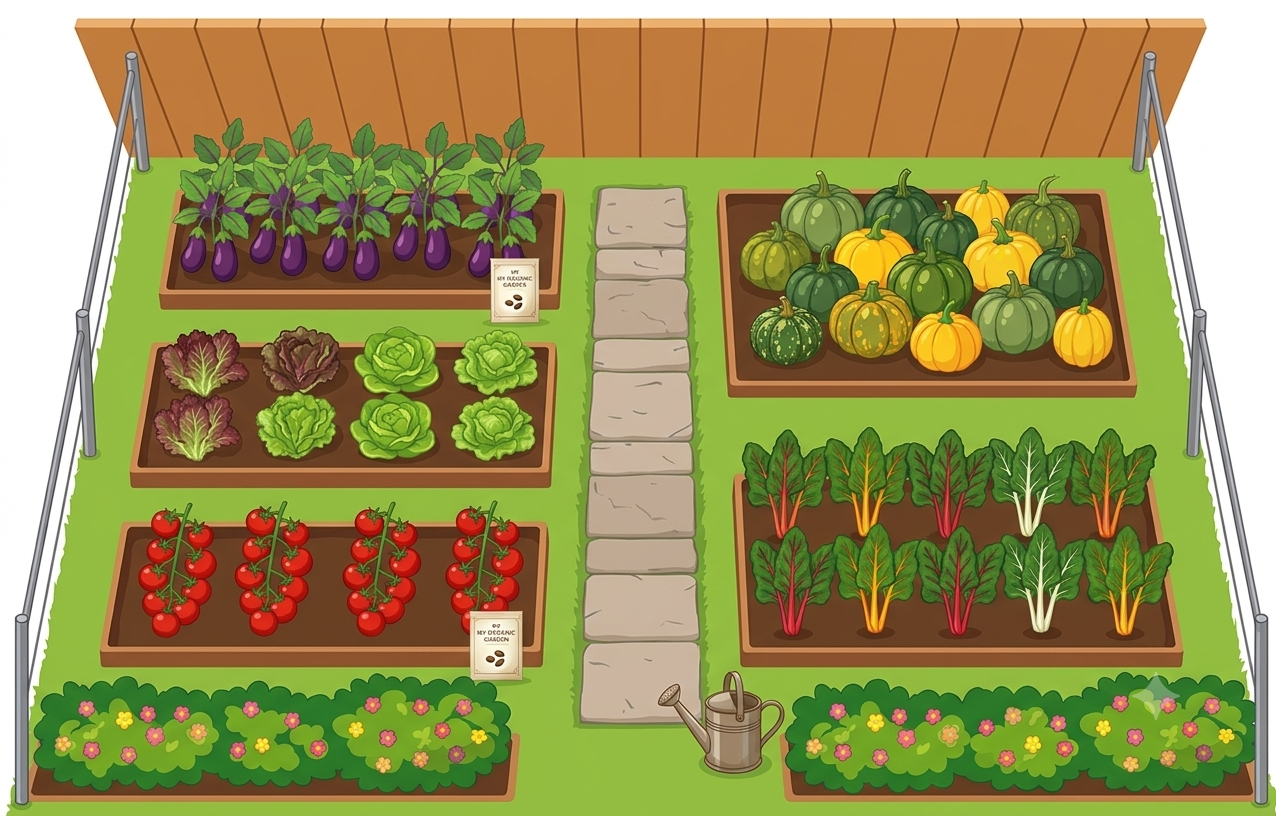
\includegraphics[width=5cm]{../images/NongTrai.png}
        };
    \end{scope}
\end{tikzpicture}
\end{center}}

% --- CÂU 25 ---
\questionShortAnswer{15}{3}{Bạn Trô Ngấu có một tấm tôn hình chữ nhật có chu vi 150cm. Bạn Trô Ngấu muốn uốn tấm tôn trên thành một hình trụ (tham khảo hình vẽ). Biết rằng bạn Trô Ngâu muốn hình trụ sau khi uốn có thể tích lớn nhất. Hỏi bạn ấy nên chọn tấm tôn hình chữ nhật có chiều dài là bao nhiêu cm?

\begin{center}
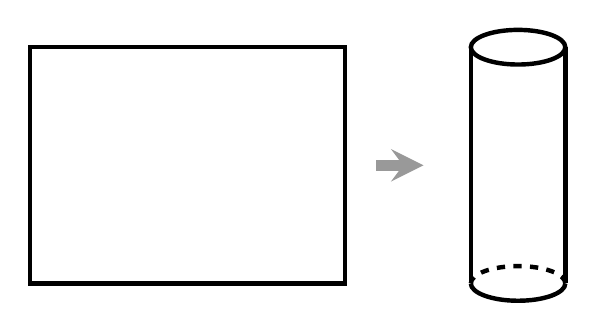
\begin{tikzpicture}[>=stealth, scale=1]

    % =================================================================
    % HÌNH BÊN TRÁI: HÌNH CHỮ NHẬT PHẲNG
    % =================================================================
    \begin{scope}[xshift=0cm, yshift=0cm]
        \draw[ultra thick] (0,0) rectangle (4,3);
    \end{scope}

    % Mũi tên chuyển bước ở giữa
    \draw[->, line width=4pt, gray!80] (4.4,1.5) -- (5.0,1.5);

    % =================================================================
    % HÌNH BÊN PHẢI: HÌNH TRỤ TRÒN (ĐÃ SỬA LỖI MẤT ĐỈNH)
    % =================================================================
    \begin{scope}[xshift=6.2cm, yshift=0cm]
        \def\R{0.6}    % Bán kính đáy elip 
        \def\H{3.0}    % Chiều cao hình trụ

        % Đáy trên: Vẽ toàn bộ bằng nét liền ôm sát hai cạnh bên
        \draw[ultra thick] (0,\H) ellipse [x radius=\R, y radius=0.22];

        % Đáy dưới: Nửa elip phía trước nét liền, nửa phía sau nét đứt
        \draw[ultra thick] (-\R,0) arc (180:360:\R\space and 0.22);
        \draw[ultra thick, dashed] (\R,0) arc (0:180:\R\space and 0.22);

        % Hai đường sinh đứng hai bên nối liền từ đáy lên đỉnh
        \draw[ultra thick] (-\R,0) -- (-\R,\H);
        \draw[ultra thick] (\R,0) -- (\R,\H);
    \end{scope}

\end{tikzpicture}
\end{center}}

% --- CÂU 16 ---
\questionShortAnswer{15}{4}{Anh 10 dự định sử dụng hết \( 6 \, m^2 \) kính để làm một bể cá bằng kính có dạng hình hộp chữ nhật không nắp, chiều dài gấp đôi chiều rộng (các mối ghép có kích thước không đáng kể). Hỏi anh 10 có thể làm được bể cá có dung tích lớn nhất bằng bao nhiêu \( m^3 \) (kết quả làm tròn đến hàng phần trăm)?}

% --- CÂU 4 ---
\questionTrueFalse{15}{5}{Bác thợ hàn dùng một thanh kim loại dài 300cm để uốn thành khung cửa sổ có dạng như hình vẽ. Gọi \( r \) là bán kính của nửa đường tròn.

\begin{center}
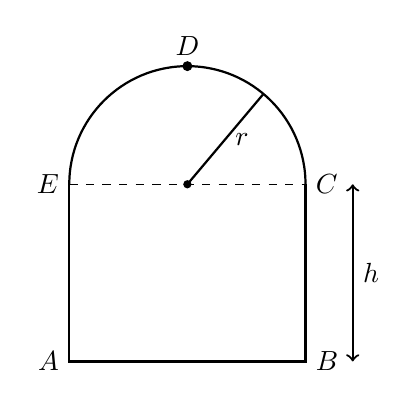
\begin{tikzpicture}[scale=1.5, thick]
        % Định nghĩa các điểm tọa độ gốc
        \coordinate (A) at (0,0);
        \coordinate (B) at (2,0);
        \coordinate (C) at (2,1.5);
        \coordinate (E) at (0,1.5);
        \coordinate (O) at (1,1.5); % Tâm của nửa đường tròn
        \coordinate (D) at (1,2.5); % Đỉnh cao nhất của nửa đường tròn

        % Vẽ khung hình chữ nhật phía dưới (khuyết cạnh trên)
        \draw (E) -- (A) -- (B) -- (C);

        % Vẽ nửa đường tròn phía trên từ điểm C đến E, tâm O, bán kính r = 1
        \draw (C) arc (0:180:1);

        % Vẽ đường đứt nét nối từ E sang C
        \draw[dashed, thin] (E) -- (C);

        % Vẽ tâm O (dấu chấm nhỏ)
        \fill (O) circle (1pt);

        % Vẽ điểm D (dấu chấm ở đỉnh đường tròn)
        \fill (D) circle (1.2pt) node[above] {$D$};

        % Vẽ bán kính r từ tâm O đến một điểm trên cung tròn (góc khoảng 50 độ)
        \draw (O) -- (1.64, 2.26) node[pos=0.5, right] {$r$};

        % Vẽ mũi tên kích thước chiều cao h bên phải
        \draw[<->] (2.4, 0) -- (2.4, 1.5) node[pos=0.5, right] {$h$};

        % Gán nhãn các đỉnh
        \node[left] at (A) {$A$};
        \node[right] at (B) {$B$};
        \node[right] at (C) {$C$};
        \node[left] at (E) {$E$};

    \end{tikzpicture}
\end{center}

}{
    \textbf{a)} & Diện tích của nửa hình tròn là \( S_1 = \dfrac{1}{2}\pi r^2 \, (cm^2) \).
    & \textcolor{amberorange}{$\bigcirc$} & \textcolor{amberorange}{$\bigcirc$} \\ \hline
    
    \textbf{b)} & Diện tích của hình chữ nhật là \( S_2 = 300r - \pi r^2 - 2r^2 \, (cm^2) \).
    & \textcolor{amberorange}{$\bigcirc$} & \textcolor{amberorange}{$\bigcirc$} \\ \hline
    
    \textbf{c)} & Khi \( r = 12 \) thì diện tích của khung cửa sổ nằm trong khoảng \( (2000; 3000) \) (đơn vị: \( cm^2 \)).
    & \textcolor{amberorange}{$\bigcirc$} & \textcolor{amberorange}{$\bigcirc$} \\ \hline
    
    \textbf{d)} & Biết \( r = r_0 \) thì diện tích của khung cửa sổ tạo thành đạt giá trị lớn nhất, khi đó \( r_0 \in (41; 42) \).
    & \textcolor{amberorange}{$\bigcirc$} & \textcolor{amberorange}{$\bigcirc$} \\
}

% --- CÂU 5 ---
\questionTrueFalse{15}{6}{Một bạn trâu muốn gò một cái thùng bằng tôn dạng hình hộp chữ nhật không nắp có đáy là hình vuông và đựng đầy được 256 lít nước. Gọi độ dài cạnh đáy của thùng là \( x \, (dm) \), chiều cao của thùng là \( h \, (dm) \).}{
    \textbf{a)} & Thể tích của thùng là \( V = x^2 h \, (dm^3) \).
    & \textcolor{amberorange}{$\bigcirc$} & \textcolor{amberorange}{$\bigcirc$} \\ \hline
    
    \textbf{b)} & Tổng diện tích xung quanh và diện tích đáy của thùng là  
    \(S(x) = x^2 + \dfrac{1024}{x} \, (dm^2).\)
    & \textcolor{amberorange}{$\bigcirc$} & \textcolor{amberorange}{$\bigcirc$} \\ \hline
    
    \textbf{c)} & Đạo hàm của hàm số \( S(x) \) là  
    \(S'(x) = 2x + \dfrac{1024}{x^2}.\)
    & \textcolor{amberorange}{$\bigcirc$} & \textcolor{amberorange}{$\bigcirc$} \\ \hline
    
    \textbf{d)} & Để gò được cái thùng mà tốn ít nguyên liệu nhất thì độ dài cạnh đáy của thùng là \( 7 \, (dm) \).
    & \textcolor{amberorange}{$\bigcirc$} & \textcolor{amberorange}{$\bigcirc$} \\
}

 

\end{document}